%% ****** Start of file apstemplate.tex ****** %
%%
%%
%%   This file is part of the APS files in the REVTeX 4.2 distribution.
%%   Version 4.2a of REVTeX, January, 2015
%%
%%
%%   Copyright (c) 2015 The American Physical Society.
%%
%%   See the REVTeX 4 README file for restrictions and more information.
%%
%
% This is a template for producing manuscripts for use with REVTEX 4.2
% Copy this file to another name and then work on that file.
% That way, you always have this original template file to use.
%
% Group addresses by affiliation; use superscriptaddress for long
% author lists, or if there are many overlapping affiliations.
% For Phys. Rev. appearance, change preprint to twocolumn.
% Choose pra, prb, prc, prd, pre, prl, prstab, prstper, or rmp for journal
%  Add 'draft' option to mark overfull boxes with black boxes
%  Add 'showkeys' option to make keywords appear
\documentclass[aps,prl,groupedaddress,amsmath,amssymb]{revtex4-2}
%\documentclass[aps,prl,preprint,superscriptaddress]{revtex4-2}
%\documentclass[aps,prl,reprint,groupedaddress]{revtex4-2}
\usepackage{graphicx}% Include figure files
\usepackage{dcolumn}% Align table columns on decimal point
\usepackage{bm}% bold math
% You should use BibTeX and apsrev.bst for references
% Choosing a journal automatically selects the correct APS
% BibTeX style file (bst file), so only uncomment the line
% below if necessary.
%\bibliographystyle{apsrev4-2}

\begin{document}

% Use the \preprint command to place your local institutional report
% number in the upper righthand corner of the title page in preprint mode.
% Multiple \preprint commands are allowed.
% Use the 'preprintnumbers' class option to override journal defaults
% to display numbers if necessary
%\preprint{}

%Title of paper
\title{\texttt{PhaseUtils}: A Python package to process and control optical fields}

% repeat the \author .. \affiliation  etc. as needed
% \email, \thanks, \homepage, \altaffiliation all apply to the current
% author. Explanatory text should go in the []'s, actual e-mail
% address or url should go in the {}'s for \email and \homepage.
% Please use the appropriate macro foreach each type of information

% \affiliation command applies to all authors since the last
% \affiliation command. The \affiliation command should follow the
% other information
% \affiliation can be followed by \email, \homepage, \thanks as well.
\author{Tangui Aladjidi}
\email[To whom correspondance should be adressed: ]{tangui.aladjidi@lkb.upmc.fr}
\affiliation{Laboratoire Kastler Brossel, Sorbonne University, CNRS, ENS-PSL University, Collège de France; 4 place Jussieu, 75005 Paris, France}
\author{Myrann Baker-Rasooli}
\affiliation{Laboratoire Kastler Brossel, Sorbonne University, CNRS, ENS-PSL University, Collège de France; 4 place Jussieu, 75005 Paris, France}
\author{Quentin Glorieux}
\affiliation{Laboratoire Kastler Brossel, Sorbonne University, CNRS, ENS-PSL University, Collège de France; 4 place Jussieu, 75005 Paris, France}

\maketitle

\section{Summary\label{summary}}

Off-axis interferometry is a powerful technique that allows full-field
retrieval from interferograms
\cite{lieblingComplexwaveRetrievalSingle2004}
\cite{verrierOffaxisDigitalHologram2011}. 
Based on the deconvolution of
the inteferograms using Fourier transforms, it allows live monitoring of
optical fields. 
It comprises of three utilities \texttt{contrast},
\texttt{velocity} and \texttt{SLM}:

\begin{itemize}
\item
  \texttt{contrast} is focused on the retrieval of the phase.
\item
  \texttt{velocity} is focused on the processing of the complex field.
\item
  \texttt{SLM} provides a performant, platform independant window-based
  tool to control spatial light modulators such as liquid crystal
  spatial light modulators (LCOS SLM) or digital micro-mirror devices
  (DMD).
\end{itemize}

\section{Statement of need}\label{statement-of-need}

Phase retrieval is a critical topic in all optics experiment. It is
often challenging since cameras can only access intensity information.
The solution to this problem is spatially heterodyning a target signal
with a reference signal using the interference signal to recover the
phase. 
This is the so-called off-axis interferometry technique
\cite{verrierOffaxisDigitalHologram2011}. 
It allows a singe shot, high
resolution retrieval of the full complex optical field.

\texttt{PhaseUtils} harnesses the power of modern FFT algorithms to
deliver performance focused tools to retrieve and process the phase
information of optical fields with its utilities \texttt{contrast} and
\texttt{velocity}. 
This allows to compute a large number of observables
relevant in the context of quantum fluids of light
\cite{aladjidiFullOpticalControl2023, glorieuxHotAtomicVapors2023,bakerrasooliTurbulentDynamicsTwodimensional2023}.
\texttt{velocity} implements all of the observables introduced in
\cite{bradleyEnergySpectraVortex2012} and implemented in the
\texttt{Julia} package
\href{https://github.com/AshtonSBradley/QuantumFluidSpectra.jl}{\texttt{QuantumFluidSpectra.jl}}
\cite{PhysRevA.106.043322}, and extends it by providing a fast
tree-based implementation of the vortex clustering algorithm.

\begin{figure}
\centering
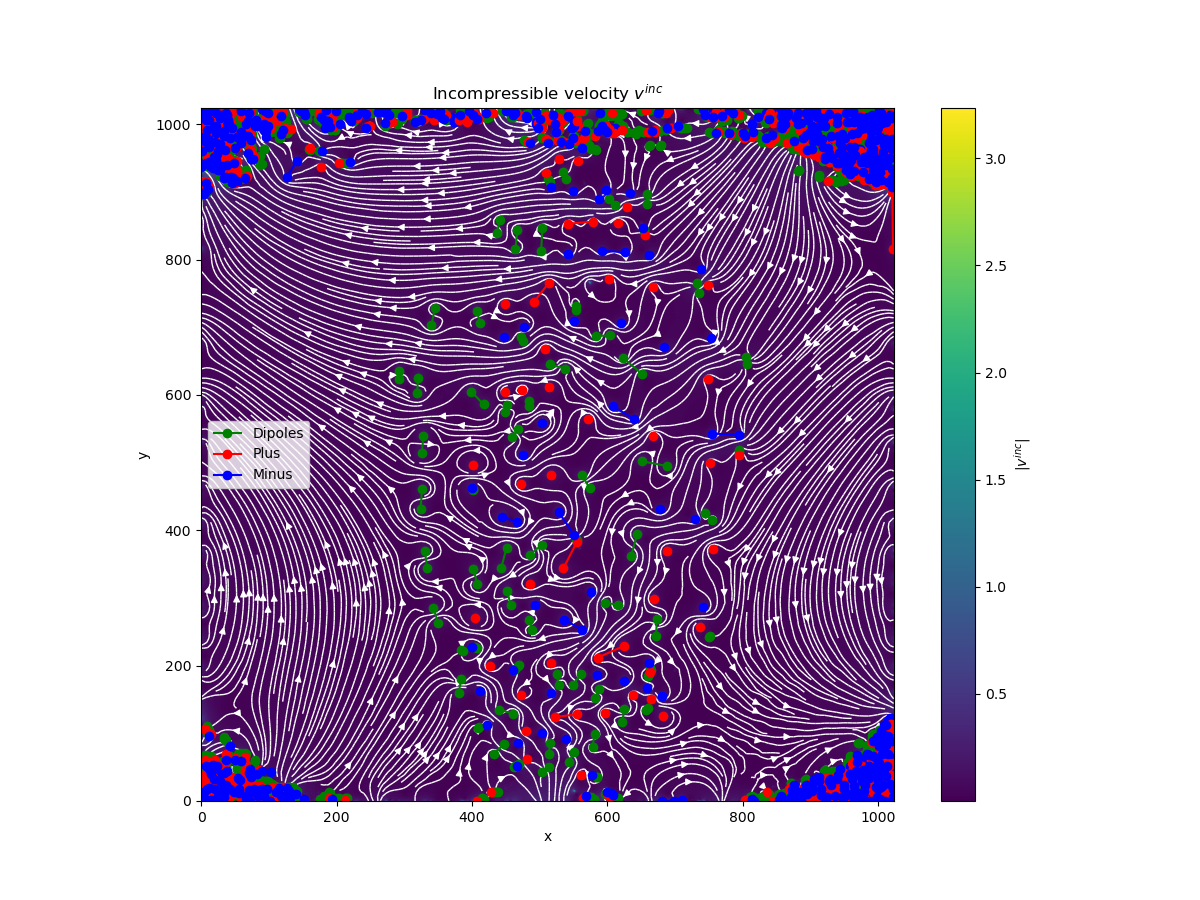
\includegraphics[width=\linewidth]{clusters.png}
\caption{Example of the vortex detection and clustering algorithm.
Positively charged vortices are in red, negatively charged vortices are
blue and dipoles are in green. The background image is the
incompressible velocity in which vortices can be seen as bright
peaks.\label{fig:clusters}}
\end{figure}

It also provide tools with \texttt{SLM} to control the optical fields
using spatial light modulators, implementing holography techniques such
as \cite{bolducExactSolutionSimultaneous2013}. 
This utility was inspired
by \cite{sebastien_m_popoff_2017_293042} and implements the same
basic functionalities, using a faster backend (\texttt{opencv}). 
Since
it functions by instantiating a graphical window, it can be used for any
spatial light modulator that is recognized as a screen. 
It also extends
the simple control functionality with all of the relevant functions to
generate arbitrary states of light using these modulators. 
These
functions use just-in-time (JIT) compilation with \texttt{numba} for optimal
performance to allow for fast live control.

\section{Acknowledgements\label{acknowledgements}}

We acknowledge the extremely meaningful conversations we had with
Riccardo Panico and Ashton Bradley. We acknowledge contributions from
Kevin Falque and constructive feedback from Clara Piekarski and Quentin
Schibler.

\section{Authors contribution\label{authors-contribution}}

T.A wrote the original code and is the main maintainer, M.B was the main
contributor on \texttt{velocity}. Q.G supervised the project.

\section{References\label{references}}

\bibliography{paper}

\end{document}